\documentclass[aps, twocolumn, floatfix, superscriptaddress]{revtex4}
\usepackage{amsmath, amssymb, amsfonts, gensymb}
\bibliographystyle{apsrev}
\usepackage{graphicx}
\graphicspath{ {Figures/} }
\newcommand{\tdc}[3][]{\frac{\mathrm{d}^{#1}#2}{\mathrm{d}#3^{#1}}} % total differential change.
\newcommand{\pdc}[3][]{\frac{\partial^{#1} #2}{\partial #3^{#1}}} % partial differential change.
\newcommand{\td}[1]{\mathrm{d}#1}
\newcommand{\pd}[1]{\partial#1}

\begin{document}

\title{Hydrodynamics of a Stationary C-boat}

\author{V. S. Akella}
\affiliation{Collective Interactions Unit, OIST Graduate University, 1919-1 Tancha, Onna-son, Okinawa, Japan 904-0495}
\author{D. K. Singh}
\affiliation{Collective Interactions Unit, OIST Graduate University, 1919-1 Tancha, Onna-son, Okinawa, Japan 904-0495}
\author{R. K. Singh}
\affiliation{School of Engineering, Brown University, 182 Hope Street, Providence, RI 02906, USA}
\author{S. Mandre}
\affiliation{School of Engineering, Brown University, 182 Hope Street, Providence, RI 02906, USA}
\author{M. M. Bandi}
\affiliation{Collective Interactions Unit, OIST Graduate University, 1919-1 Tancha, Onna-son, Okinawa, Japan 904-0495}
\email[Corresponding Author: ]{bandi@oist.jp}

\date{\today}

\begin{abstract}
In the present work, we attempt to understand the hydrodynamics associated with a \emph{c-boat} held fixed at the air-water interface. A \emph{c-boat} is a disc-shaped agarose gel tablet with all the water in the agarose gel replaced by camphoric acid. Camphoric acid spreads over the air-water interface due to the interfacial tension between forces. The spread radius grows as power law in time with a scaling exponent of $\frac{1}{2}$, in agreement with observed scaling for the time-dependent spread radius for other volatile substances at the air-water interface. As camphoric acid spreads, shear stresses caused by the Marangoni forces lead to the development of boundary layer at the air-water interface. Using boundary layer approximation, we derived a scaling law which shows that the fluid velocity in the boundary layer scales as a power law in distance with a scaling exponent of $-\frac{3}{5}$ and is experimentally verified. 
\end{abstract}

\maketitle
\section{Introduction}
\section{Experimental Section}
\subsection{Materials and Methods}
\label{sec:prep}
A \emph{c-boat} is a disc-shaped agarose gel tablet, with all the water in the agaorse gel matrix replaced with camphoric acid. The identical nature of c-boats is of crucial importance if one wishes to characterize/study a collection of c-boats. Note that, all the experiments in this research work are carried out with c-boats of $3\ \mathrm{mm}$ diameter and $1\ \mathrm{mm}$ thickness. The preparation of the c-boats involves the following steps. 
\begin{enumerate}
\item Preparation of 5\% w/v agarose (Wako Pure Chemical Industries, Ltd., Cat. No. 346-00072) gel sheets of uniform thickness.
\item Punching out (using Biopunch, Ted Pella, Inc.) discs of agarose gel of required disc diameter. 
\item Soaking the agarose discs in camphoric acid (Wako Pure Chemical Industries, Ltd., Cat. No. 036-01002) saturated methanol (Wako Pure Chemical Industries, Ltd., Cat. No. 138-01836) solution for more than 2 hrs. This process replaces the water from the agarose gel with camphoric acid saturated methanol solution. 
\item Washing and rinsing of the discs in de-ionized water (obtained from Milli-Q Integral Water Purification System with resistivity, $\rho=\mathrm{18\ M} \Omega\ \mathrm{cm}$ at 25 $\celsius$). This step results in (1) the evaporation of methanol and (2) the precipitation of camphoric acid in the agarose gel matrix.
\end{enumerate}
When needed, we used Sodium Dodecyl Sulfate (Wako Pure Chemical Industries, Ltd., Cat. No. 196-08675) to modify the air-water interfacial tension.
\label{sec:expset}
\begin{figure}[ht]
    \begin{center}
       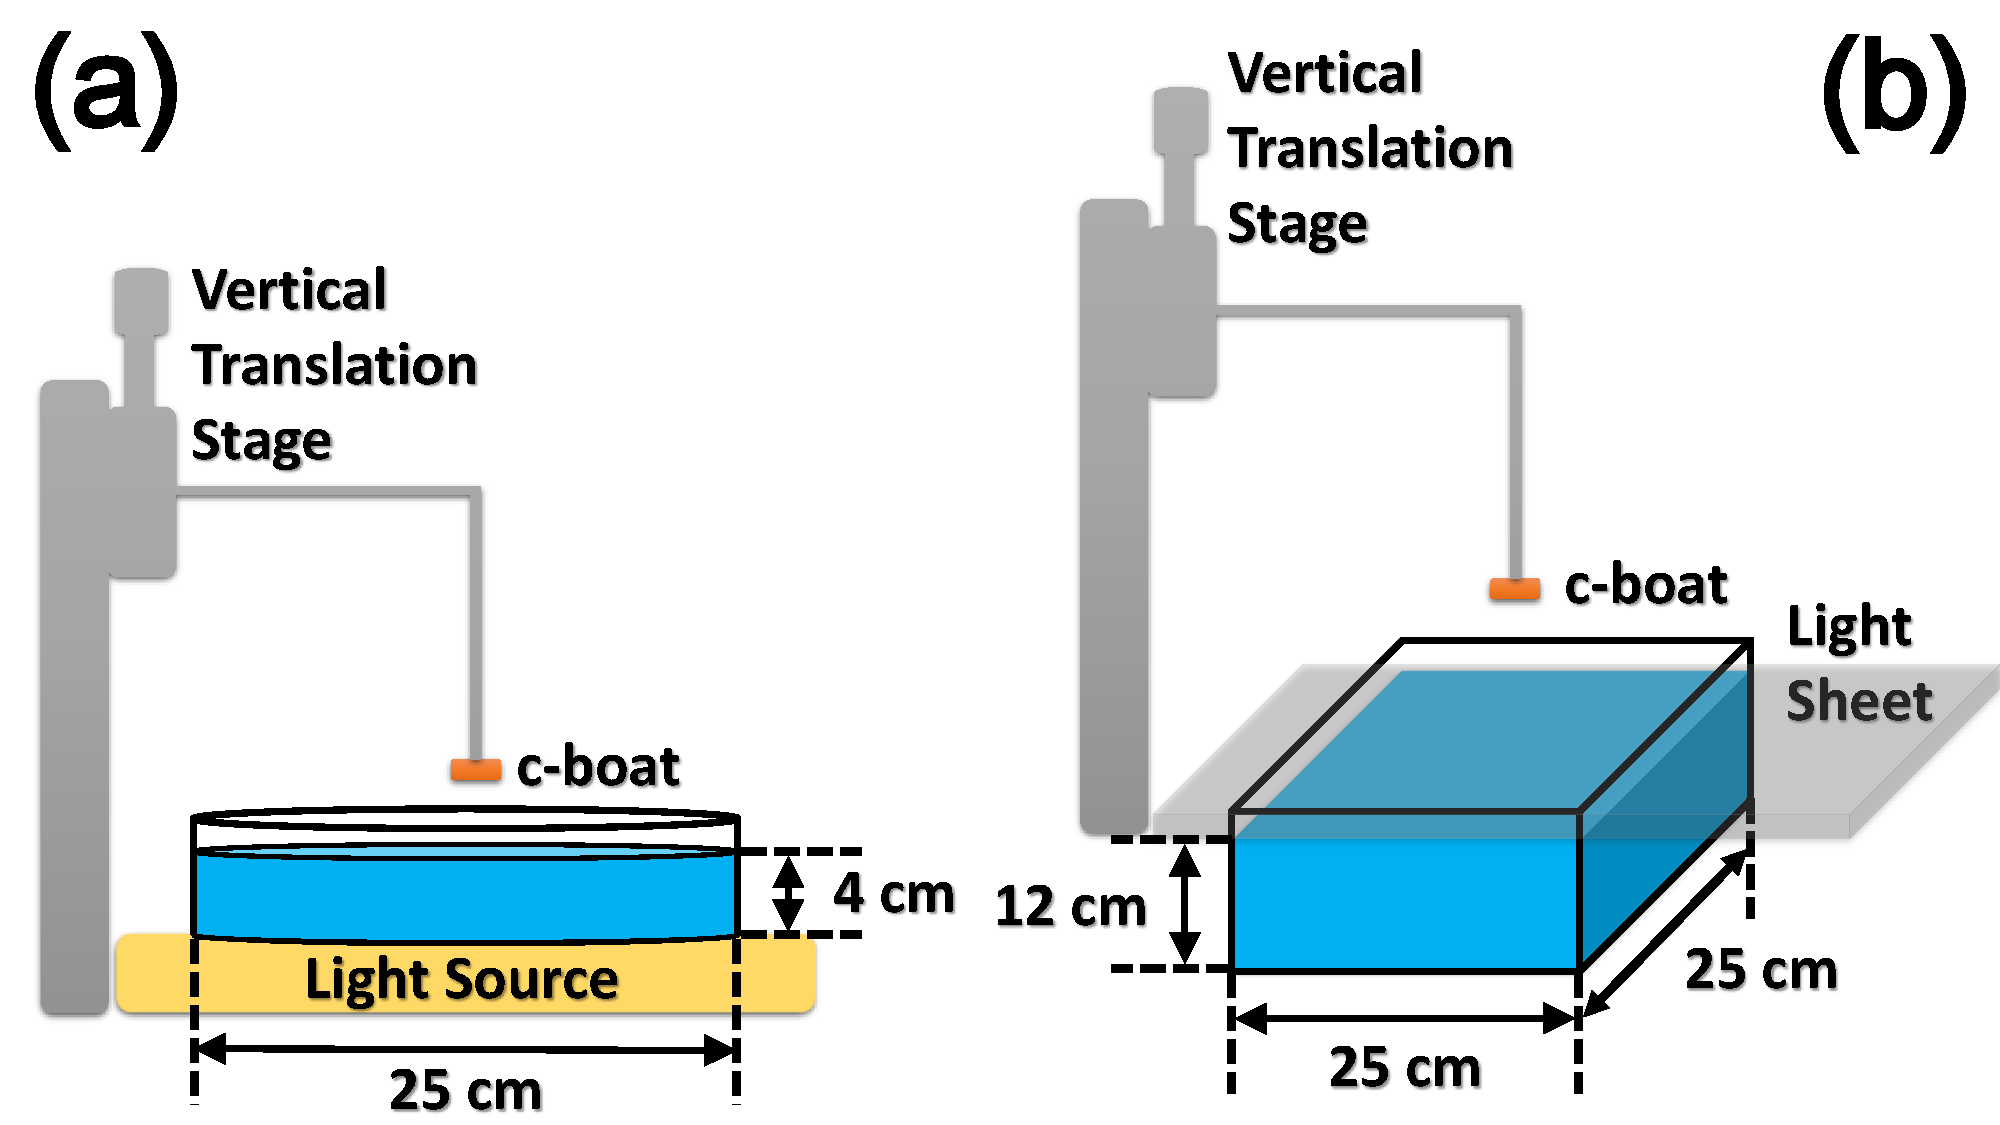
\includegraphics[scale=0.25]{figure1.pdf}
    \end{center}
    \caption{Experimental Setup.}
    \label{fig:expset}
\end{figure}
\subsection{Data Acquisition and Analysis}
The experimental setup (figure~\ref{fig:expset}) consists of (1) a glass container filled with de-ionized water (2) an L-shaped steel wire with one end firmly attached to a vertical translation stage (3) an illumination source and (4) Phantom v641 hi-speed camera, located directly above the glass container. The c-boat is attached at the free-end of the steel wire. At the beginning of the experiment the steel-wire-arrangement is lowered using the tranlational stage such that the c-boat gently makes a contact with the air-water interface and for the rest of the experiment the c-boat is left un-disturbed. For the transient regime experiments (figure~\ref{fig:expset}a), we used a 25 $\mathrm{cm}$ diameter and 5 $\mathrm{cm}$ height glass petri dish filled with approximately 2 liters of de-ionized water and the petri dish is illuminated using a light tablet from bottom. To visualize the spread dynamics, the air-water interface is covered with hydrophilic tracer particles ($d = 50\ \mu \mathrm{m}$, specific gravity = 0.25) at low packing fractions, $\phi \leq 0.2$. We did \emph{not} observe any effect of tracer particles on the spread dynamics at packing fractions, $\phi \leq 0.2$. The spread dynmics are recorded at 1000 frames per second with 100 $\mu \mathrm{s}$ exposure time using the hi-speed camera. As the camphoric acid spreads over the interface, the tracer particles are pushed away radially outwards creating a particle-free zone. The radius of the particle-free zone is measured manually from a time series of images (using ImageJ). Figure~\ref{fig:cspreadimg} shows the particle-free zone at an instant in time. For the steady state regime experiments (figure~\ref{fig:expset}b), we used a glass container of dimensions 25 $\mathrm{cm}$ $\times$ 25 $\mathrm{cm}$ $\times$ 25 $\mathrm{cm}$ filled with approximately 8 liters of de-ionized water and the air-water interface is illuminated with a laser sheet of thickness $\approx$ 3 $\mathrm{mm}$ such that the bulk layers are minimally illuminated. The fluid velocity at the interface is measured by mixing un-measurably small quantity of neutrally buoyant tracer particles ($d < 10\ \mu \mathrm{m}$). The motion of the tracer particles is recorded at 300 frames per second with 1 $\mathrm{ms}$ exposure time using the hi-speed camera. Figure~\ref{fig:radvelimg} is a resultant image obtained by adding 30 consecutive frames. The lengths of the streaks are manually measured (using ImageJ). The length of the streak, $\td{r}$ (figure~\ref{fig:radvelimg}) is the distance in centimeters (converted to centimeters using appropriate pixel to centimeter conversion factor) traveled by the tracer particle in $\td{t}=$ 0.1 $\mathrm{sec}$ at a radial distance $r$ (figure~\ref{fig:radvelimg}) from the center of the c-boat. 

\begin{figure}[ht]
\centering
  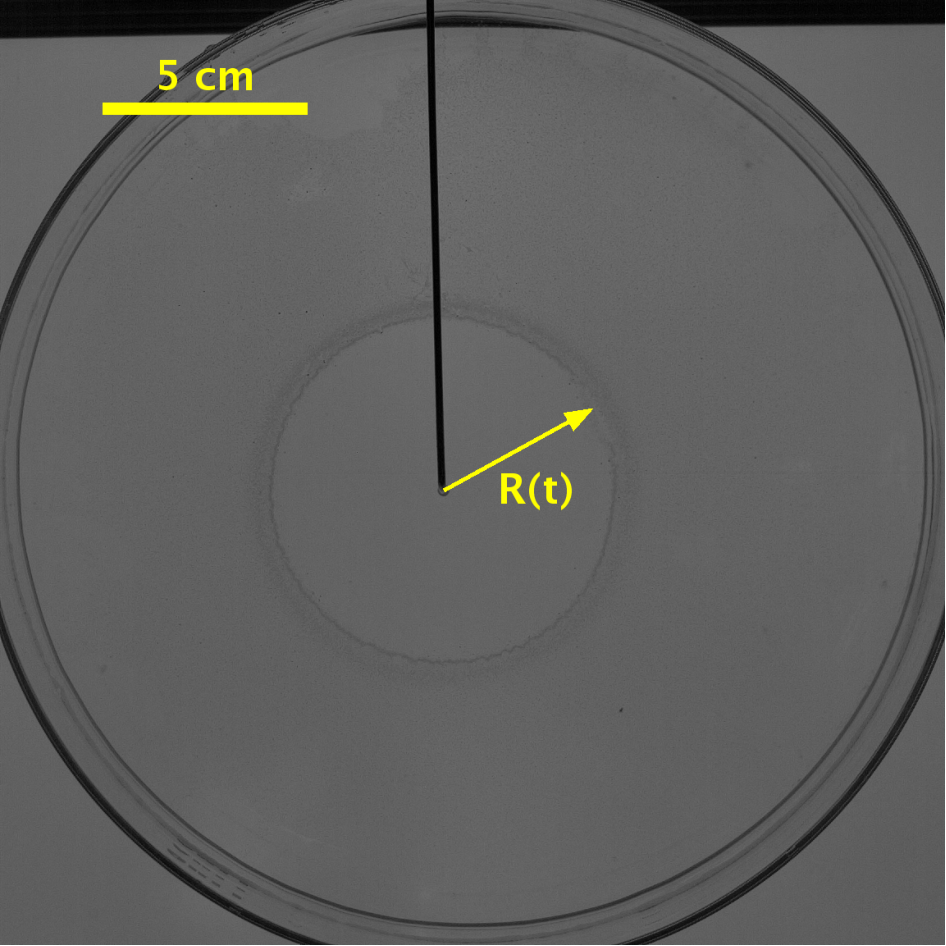
\includegraphics[width=0.8\columnwidth]{figure2.pdf}
  \caption{Caphoric acid spread radius at an instant in time, visualized using hydrophilic tracer particles.}
  \label{fig:cspreadimg}
\end{figure}
\begin{figure}[ht]
  \centering
  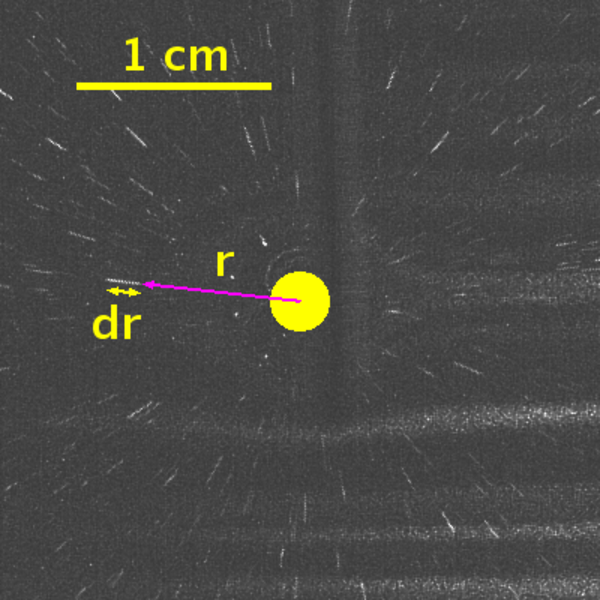
\includegraphics[width=0.8\columnwidth]{figure3.pdf}
  \caption{Measurement of radial velocity at a distance $r$ from the center of the c-boat. The length of the streak, $\td{r}$ is the distance traveled by the tracer particle in time $\td{t} = 0.1\ \mathrm{sec}$}
       \label{fig:radvelimg}
\end{figure} 

\section{Results and Discussion}
When a c-boat is placed at the air-water interface, camphoric acid is drawn out of the c-boat by the interfacial tension forces to minimize the interfacial free energy and the camphoric acid front emanates radially outwards. Due to the evaporation/sublimation of camphoric acid, the spreading can \emph{not} continue until interface is saturated with the camphoric acid. Owing to the slower evaporation/sublimation kinetics of camphoric acid compared to the spread dynamics, the concentration front spreads to a farther distance than \emph{the steady state distance}. The \emph{steady state distance} is defined as the distance, measured from the center of the c-boat, at which the advection flux and the evaporation flux of camphoric acid balance each other. As a result, the concetration front retraces to the steady state distance (see movie S1 in the supplementary information). Note that, the hydrophilic tracer particles trace back because by spreading they minimize the interfacial energy of air-water interface. For brevity, we discuss our findings in two parts, 1. The transient regime and 2. The steady state regime. 
\subsection{Transient Regime}
\label{sec:transient}
The transient regime is observed from the instance of c-boat's contact with the air-water interface to the time when the camphoric acid spread radius reaches a steady state value. During the transient regime, we observe two spreading stages (1) the divergent stage: during which the camphoric acid molecules are drawn out of the c-boat and spread radially outwards over the interface soon after the c-boat's contact with the air-water interface (2) the convergent stage: during which the spread radius shrinks to the steady state value due to evaporation/sublimation of camphoric acid. The spread radius, measured during the divergent stage, follows a power law in time with a scaling exponent of $t^{1/2}$ which is in agreement with the observed scaling for the spread of volatile oils at the air-water interface (ref). Note that, this is \emph{not} the observed scaling with non-volatile oils, for which the spread radius scales with time as $t^{3/4}$ (ref). Figure~\ref{fig:caspread} is a plot of the spread radius $R(t)$ as a function of time measured during divergent stage. We attribute the scatter in the data around the fit to the experimental variation in the depth of c-boat sitting below the air-water interface.   

\begin{figure}[ht]
    \begin{center}
       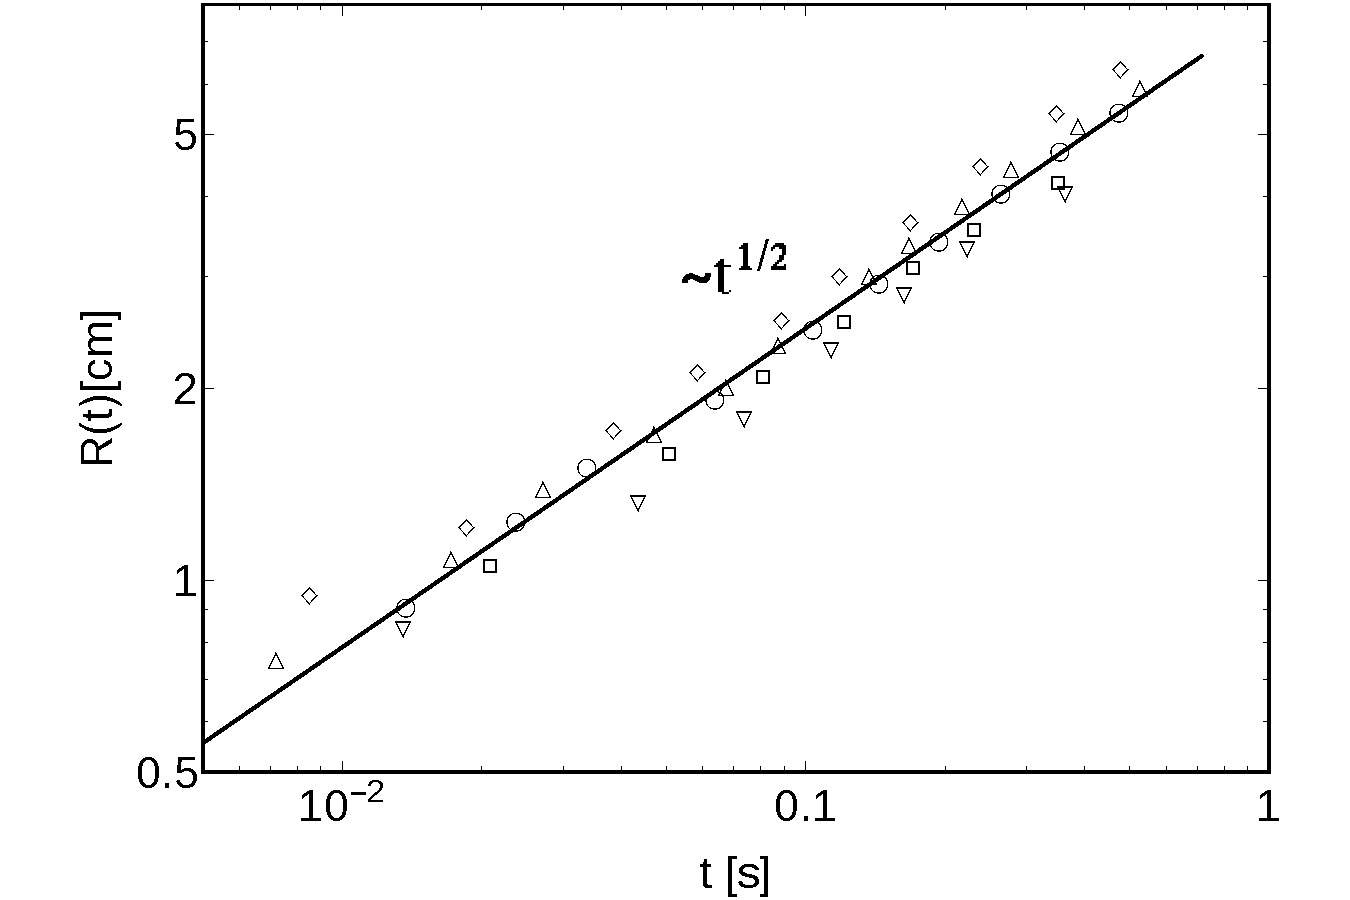
\includegraphics[scale=0.35]{figure4.pdf}
    \end{center}
    \caption{Camphoric acid radial spread vs. time. The radial front is visualized using 50 $\mu m$ hydrophilic tracer particles sparsely sprinkled at the air-water interface. }
    \label{fig:caspread}
\end{figure}

\subsection{Steady State Regime}
\label{sec:steady}
The spread of camphoric acid over the air-water interface reaches a steady state when the advection flux equals the evaporation flux. The radial distance, measured from the center of c-boat, at which the flux balance is achieved happens to be smaller than the maximum spread distance measured in the divergent stage (explained in section~\ref{sec:transient}) because of slower evaporation/sublimation kinetics than the spread dynamics. Note that, camphoric acid poorly dissolves in water and the amount of camphor entering the bulk water is negligible. However, the camphoric acid adsorbed at the air-water interface is sufficient enough to change the interfacial tension of air-water interface. As a result camphoric acid concentration gradients are setup around the c-boat. These concetrations gradients lead to the interfacial tension gradients and are the source of solutal Marangoni forces. When there is no evaporation, the spread dynamics \emph{never} reach a steady state. Note that, in a finite-sized system the spread dynamics reach a steady state when the air-water interface is saturated with the non-volatile oil. However, there will \emph{not} be concetration gradients to drive fluid flow are \emph{never} setup since there is no evaporation. Therefore, evaporation is a very critical requirement in our analysis. The Marangoni froces shear the air-water interface and cause the underlying fluid flow. The fluid flow penetrate into bulk due to the viscosity of the bluk fluid. We derive a scaling law for the radial velocity of the fluid flow at the air-water interface by invoking the boundary layer approximation. Let $c(r)$ and $u(r)$ be the radial concentration and velocity profiles at the air-water interface. Then the flux of camphor $q$ at a radial distance $r$ is: 
\begin{equation}
q \approx r u_{r} c \implies c \approx \frac{q}{ru_{r}} 
\end{equation}
Assumption:
\begin{align}
u(r, z) &= r^{n} f\left( \frac{z}{\delta(r)} \right) \\
u_{z} = \pdc{u}{z} &= \frac{r^{n}}{\delta(r)} f^{\prime}\left(\frac{z}{\delta(r)} \right)
\end{align}
Order of magnitude estimation yields:
\begin{equation}
C = \frac{Q}{RU_{r}}
\end{equation}
Assuming that intefacial tension $\sigma (r)$ varies linearly with concentration $c(r)$. The solutal Marangoni force is:
\begin{equation}
\sigma (r) = -k_{1} c(r) + \sigma_{0} \implies \tdc{\sigma}{r} = -k_{1}\tdc{c}{r}  \approx k \frac{C}{R}
\end{equation}
where, $k_{1}$ is the proportionality constant. 
Boundary layer approximation and continuity equation yield: 
\begin{align}
u_{r}\pdc{u_{r}}{r} + u_{z}\pdc{u_{r}}{z} &= \nu \pdc[2]{u_{r}}{z} \\
\pdc{(ru_{r})}{r} + r\pdc{u_{z}}{z} &= 0
\end{align}
Order of magnitude calculations yield:
\begin{align}
\frac{U_{r}^{2}}{R} \approx \frac{U_{r}U_{z}}{\delta} &\approx \frac{\nu U_{r}}{\delta^{2}} \\ 
\frac{U_{r}}{R} &\approx \frac{U_{z}}{\delta} 
\end{align}
Simplifying above equations yield:
\begin{equation}
\delta = \sqrt{\frac{\nu R}{U_{r}}}
\end{equation}
At the air-water interface, the Marangoni stresses are balanced by the viscous stresses. Mathematically,
\begin{equation}
k_{1}\tdc{c}{r} = \mu \tdc{u_{r}}{z} \implies \frac{k_{1}C}{R} = \frac{\mu U_{r}}{\delta}
\end{equation}
Substituting equations (??) and (??) 
\begin{equation}
\frac{k_{1}Q}{U_{r}R^{2}} = \frac{\mu U_{r}}{\sqrt{\frac{\nu R}{U_{r}}}} \implies
\boxed{U_{r} = \left(\frac{k_{1}Q\nu^{1/2}}{\mu}\right)^{2/5} R^{-3/5}}
\end{equation}
\begin{figure}[ht] 
    \begin{center}
       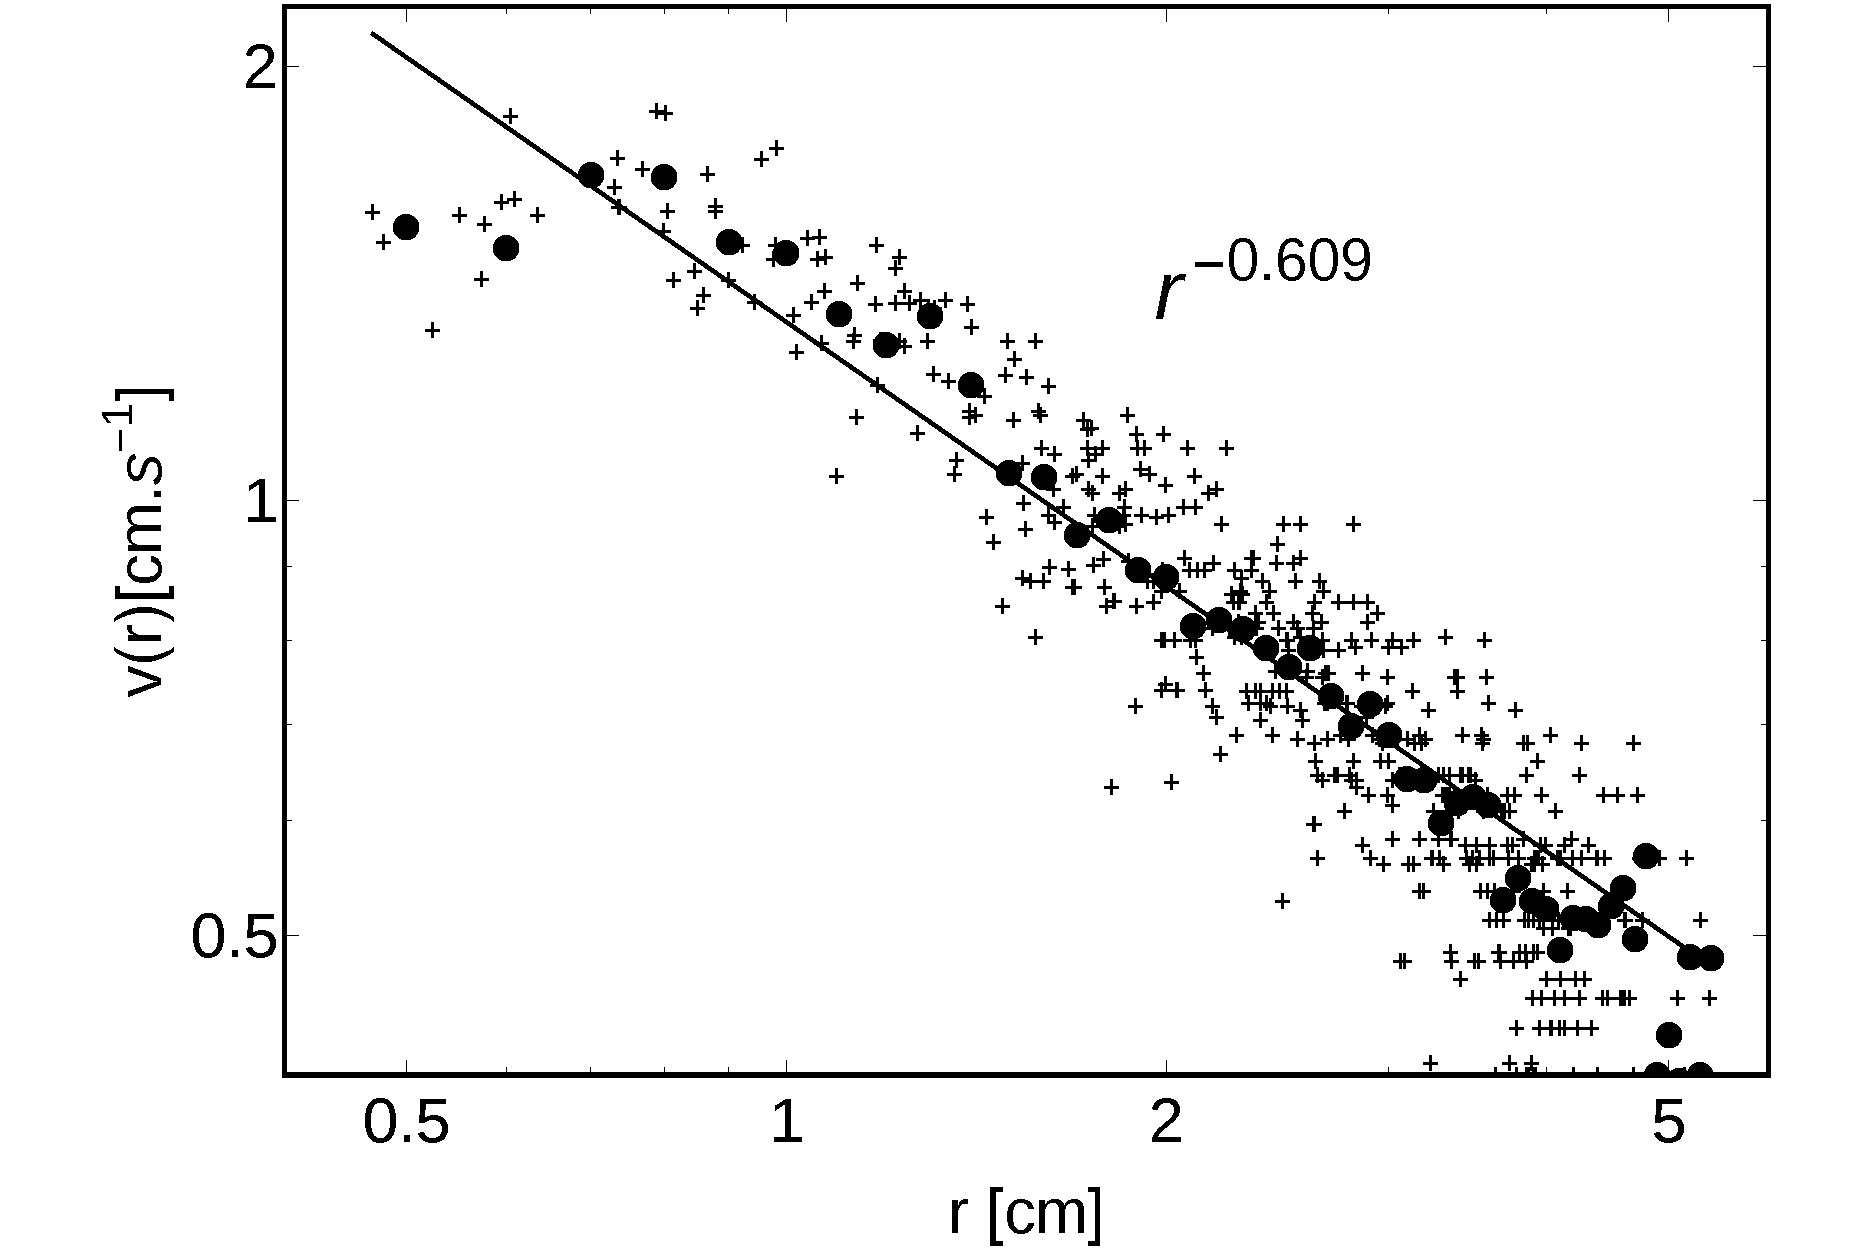
\includegraphics[scale=0.25]{figure5.pdf}
    \end{center}
    \caption{Radial velocity measured at the air-water interface}
    \label{fig:radvel}
\end{figure}

\section{Summary}
\label{sec:summary}
When a c-boat is held fixed at the air-water interface, camphoric acid molecules are drawn on to the air-water interface. The camphoric acid molecueles spread over the interface to minimize the air-water interfacial energy. The spread radius follows a $t^{1/2}$ power law scaling in time and is in agreement with similar observations on non-volatile oils. The system reaches a steady state when there is a balance between the advection flux and evaporation flux of camphoric acid molecules. The adsorbed camphoric acid molecules modify the air-water interfacial tension. These interfacial tension gradients shear the air-water interface causing the underlying fluid to flow, known as solutal Marangoni flow. We derived a scaling law for the radial velocity of the shear flow at the air-water interface as function of radial distance by invoking the boundary layer approximation. The derived scaling law is: $u(r) \propto r^{-3/5}$ where $u(r)$ is the radial velocity at the interface and $r$ is the radial distance measured from the center of the c-boat. Moreover, we experimentally confirmed that the radial velocity indeed agrees with the proposed scaling law as a function of radial distance.       
\acknowledgments
VSA, DKS, SB and MMB were supported by the OIST Graduate University with subsidy funding from the Cabinet Office, Government of Japan. RKS was hosted by OIST Graduate University on a research internship while performing this work. MMB acknowledges L. Mahadevan for introducing the camphor boat system and subsequent scientific discussions, and D. Vu Anh for help with preliminary experiments.

\bibliography{all}

\end{document} 
